%\begin{center}
%\textbf{
%%\dots
%\og 
%Rentrée Pastorale 2025-2026
%\fg{}
%%\dots
%}
%\end{center}

%Une nouvelle rentrée pastorale qui nous réjouit tous. En effet, après un temps de répit, il nous revient de mettre en marche la machine de nos activités pastorales.

Au début de cette nouvelle année pastorale, je souhaite vous redire toute ma joie de vous retrouver pour continuer la mission qui m’est assignée dans notre communauté de paroisses. Et comme chaque année, nous mettrons l’accent en premier lieu sur la vie catéchétique des enfants et des adolescents,
l’animation liturgique, la création d’une troisième chorale, la visite aux malades et dans notre maison de retraite (\emph{Résidence du Parc}), l’accueil et l’accompagnement en vue de baptêmes,  du catéchuménat des adultes, des mariages, l’encadrement  des servants d’autel, l’entretien de notre église pour la rendre  accueillante, avec ces innombrables petits gestes de service qui jalonnent l’existence ; tout cela nous aidera à vivre une véritable dimension ecclésiale. 

%Je voudrais vous remercier de tout cœur, vous tous qui êtes des membres vivants et actifs de la communauté paroissiale que nous formons, véritable artisans de l’évangélisation ordinaire. Mon souhait pour la vie de notre communauté de paroisses est que nous arrivions toujours plus à nous ouvrir et à nous connaître les uns les autres, à nous apprécier dans ce que nous sommes et vivons.

%L’année dernière, avec toutes les entités de nos deux paroisses, nous avons eu différentes propositions, activités et invitations qui ont favorisées l’\textbf{Unité et l’ouverture} qui constituaient notre thème pastoral. Ne manquons pas cette année ces moments simples et conviviaux qui permettent de tisser des liens gratuits, profonds et tout simplement chrétiens.

Cette année nous porterons ensemble cette rentrée dans le cœur de chacun avec nos \textbf{jeunes pro}. Chacun à son rythme, selon ses possibilités et ses réalités mais avec un seul et même objectif : l’accomplissement de nos activités communautaires. Présentons également notre rentrée paroissiale au Christ. Et continuons notre chemin pour la mise en œuvre de notre projet paroissial autour de ce principal thème :
\textbf{\og Avec notre jeunesse bâtissons une communauté plus dynamique, rayonnante et missionnaire \fg{}}.

%\begin{wrapfigure}{l}{1.0cm}
%\vspace{-0.4cm}
%	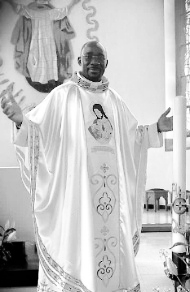
\includegraphics[scale=1.20]{../images/standing_daniel}
%\end{wrapfigure}
En ce dimanche de la fête de la Croix Glorieuse, fête patronale de notre paroisse de Sainte Croix, nous sommes invités par le Christ notre Rédempteur à déposer au pied de sa croix tous nos fardeaux, nos soucis, nos difficultés, nos épreuves et notre égo. Avec le Christ, la croix devient la clé qui ouvre la porte de nos prisons et brise toutes les chaines qui nous aliènent. En nous inscrivant dans cette espérance, allons tous témoigner avec nos jeunes auprès de tous ceux qui n’espèrent plus que le Christ vainqueur de la mort veut nous entrainer dans son élévation.

%Que cette rentrée pastorale nous aide à prendre des résolutions nécessairement pour plonger à frais nouveaux dans la parole et être des disciples crédibles de l’évangile.


\begin{flushright}
Belle rentrée à tous.
\textit{Père  Daniel  ETTÉ}
\end{flushright}

